% For copyright and license information, see uiucthesis2021.dtx and derivatives.
\documentclass{uiucthesis2021}
\usepackage[utf8]{inputenc}
\usepackage[english]{babel}
\usepackage{csquotes}
\usepackage{microtype}
\usepackage{amsmath,amsthm,amssymb}
\usepackage[bookmarksdepth=3,linktoc=all,colorlinks=true,urlcolor=blue,linkcolor=blue,citecolor=blue]{hyperref}
\usepackage[capitalize]{cleveref}
\usepackage[style=ieee, dashed=false]{biblatex}

% Added packages
\usepackage{graphicx}
\usepackage{relsize}
\usepackage{array}
\usepackage{listings}
% \usepackage{caption}
\usepackage[justification=centering]{caption}
\usepackage{subcaption}
\usepackage{booktabs}
\usepackage{multirow}
\usepackage{algorithm}
\usepackage[noend]{algpseudocode}
\usepackage{csvsimple}
\usepackage{longtable}
\usepackage[acronym,toc]{glossaries}

% \usepackage{ruledchapters}  % example of compliant heading format, uncomment to use

\usepackage{lipsum}  % just for placeholder code

% uncomment the below to show a grid on all pages
% \usepackage[grid, gridunit=in, gridcolor=blue!40, subgridcolor=blue!20]{eso-pic}

%%%%%%%%%%%%%%%%%%%%%%%%%%%%%%%%%%%%%%%%%%%%%%%%%%%%%%%%%%%%%%%%%%%%%%%%%%%%%%%
\addbibresource{./references.bib}

\newcounter{counterforappendices}

%%%%%%%%%%%%%%%%%%%%%%%%%%%%%%%%%%%%%%%%%%%%%%%%%%%%%%%%%%%%%%%%%%%%%%%%%%%%%%%
\begin{document}

\title{A Reactor Physics Framework to Detect Anomalies in HTGR Core}
\author{Harun Ardiansyah}
\department{Nuclear, Plasma, and Radiological Engineering}
%\concentration{Coffee Studies}
\phdthesis
\degreeyear{2025}
\committee{
    Professor Tomasz Kozlowski, Director of Research, Chair\\
    Professor Angela Di Fulvio\\
    Assistant Professor Syed Bahauddin Alam\\
    Professor Eduard-Wilhelm Kirr\\
    Professor Christophe Demazière}
\maketitle

%%%%%%%%%%%%%%%%%%%%%%%%%%%%%%%%%%%%%%%%%%%%%%%%%%%%%%%%%%%%%%%%%%%%%%%%%%%%%%%
\frontmatter

\newacronym{AGR1}{AGR-1}{Advanced Gas Reactor 1}
\newacronym{ANL}{ANL}{Argonne National Laboratory}
\newacronym{ANN}{ANN}{Artificial Neural Network}
\newacronym{API}{API}{Application Programming Interface}
\newacronym{ATR}{ATR}{Advanced Test Reactor}
\newacronym{B4C}{B4C}{boron carbide}
\newacronym{BC}{BC}{boundary condition}
\newacronym{BOC}{BOC}{beginning of the equilibrium cycle}
\newacronym{BNCT}{BNCT}{Boron Neutron Capture Therapy}
\newacronym{BSD}{BSD}{Berkeley Software Distribution}
\newacronym{BWR}{BWR}{Boiling Water Reactor}
\newacronym{CAISO}{CAISO}{California ISO}
\newacronym{CAPP}{CAPP}{Core Analyzer for Pebble and Prism type VHTRs}
\newacronym{CEA}{CEA}{Commissariat a l'Energie Atomique}
\newacronym{CFD}{CFD}{computational fluid dynamics}
\newacronym{CO2}{CO$_2$}{carbon dioxide}
\newacronym{CNN}{CNN}{Convolutional Neural Network}
\newacronym{CR}{CR}{control rod}
\newacronym{CRAM}{CRAM}{Chebyshev Rational Approximation Method}
\newacronym{CRP}{CRP}{Coordinated Research Project}
\newacronym{CZP}{CZP}{Cold Zero Power}
\newacronym{DCC}{DCC}{depressurized conduction cool-down}
\newacronym{DOD}{DOD}{U.S. Department of Defense}
\newacronym{DOE}{DOE}{Department of Energy}
\newacronym[\glslongpluralkey={degrees of freedom}]{DoF}{DoF}{degree of freedom}
\newacronym{DT}{DT}{Decision Tree}
\newacronym{DTR}{DTR}{Decision Tree Regression}
\newacronym{EOC}{EOC}{end of the equilibrium cycle}
\newacronym{FCEV}{FCEV}{Fuel Cell Electric Vehicle}
\newacronym{FDM}{FDM}{Finite Difference Method}
\newacronym{FEM}{FEM}{Finite Element Method}
\newacronym{FNN}{FNN}{Feedforward Neural Network}
\newacronym{FVM}{FVM}{Finite Volume Method}
\newacronym[\glslongpluralkey={greenhouse gases}]{GHG}{GHG}{greenhouse gas}
\newacronym[\glslongpluralkey={Gaussian processes}]{GP}{GP}{Gaussian process}
\newacronym{GRS}{GRS}{Gesellschaft für Anlagen und Reaktorsicherheit}
\newacronym{GT-MHR}{GT-MHR}{Gas Turbine-Modular Helium Reactor}
\newacronym{H2}{H$_2$}{hydrogen}
\newacronym{He}{He}{helium}
\newacronym{HFIR}{HFIR}{High Flux Isotope Reactor}
\newacronym{HFP}{HFP}{Hot Full Power}
\newacronym{HPC}{HPC}{high-performance computing}
\newacronym{HPCC}{HPCC}{high-pressure conduction cool-down}
\newacronym{HTE}{HTE}{High-Temperature Electrolysis}
\newacronym{HTGR}{HTGR}{High-Temperature Gas-Cooled Reactor}
\newacronym{HTR}{HTR}{High Temperature Reactor}
\newacronym{HTTR}{HTTR}{High-Temperature engineering Test Reactor}
\newacronym{HZDR}{HZDR}{Helmholtz-Zentrum Dresden-Rossendorf}
\newacronym{IAEA}{IAEA}{International Atomic Energy Agency}
\newacronym{icap}{iCAP}{Illinois Climate Action Plan}
\newacronym{INL}{INL}{Idaho National Laboratory}
\newacronym{IPyC}{IPyC}{inner pyrolytic carbon}
\newacronym{IRIS}{IRIS}{International Reactor Innovative and Secure}
\newacronym{ITER}{ITER}{International Thermonuclear Experimental Reactor}
\newacronym{JFNK}{JFNK}{Jacobian-Free Newton-Krylov}
\newacronym{KAERI}{KAERI}{Korea Atomic Energy Research Institute}
\newacronym{Keff}{k$_{eff}$}{multiplication factor}
\newacronym{KNN}{KNN}{K-Nearest Neighbors}
\newacronym{LANL}{LANL}{Los Alamos National Laboratory}
\newacronym{LBP}{LBP}{Lumped Burnable Poison}
\newacronym{LEU}{LEU}{low-enriched uranium}
\newacronym{HEU}{HEU}{highly-enriched uranium}
\newacronym{LGPL}{LGPL}{Lesser GNU Public License}
\newacronym{LOCA}{LOCA}{loss-of-coolant accident}
\newacronym{LOFW}{LOFW}{loss-of-feedwater}
\newacronym{LOFA}{LOFA}{loss-of-flow accident}
\newacronym{LogR}{LogR}{Logistic Regression}
\newacronym{LPCC}{LPCC}{low-pressure conduction cool-down}
\newacronym{LR}{LR}{Linear Regression}
\newacronym{LSTM}{LSTM}{Long Short-Term Memory Network}
\newacronym{LTE}{LTE}{Low-Temperature Electrolysis}
\newacronym{LWR}{LWR}{Light Water Reactor}
\newacronym{MOAA}{MOAA}{MCNP-ORIGEN Activation Automation}
\newacronym{MC}{MC}{Monte Carlo}
\newacronym{MHTGR}{MHTGR}{Modular High-Temperature Gas-Cooled Reactor}
\newacronym{ML}{ML}{machine learning}
\newacronym{MMR}{MMR}{Micro Modular Reactor}
\newacronym{MOC}{MOC}{middle of the equilibrium cycle}
\newacronym{MOX}{MOX}{Mixed-Oxide}
\newacronym{MOOSE}{MOOSE}{Multi-physics Object-Oriented Simulation Environment}
\newacronym{MPI}{MPI}{Message Passing Interface}
\newacronym{MAE}{MAE}{Mean Absolute Error}
\newacronym{MSE}{MSE}{Mean Squared Error}
\newacronym{MSR}{MSR}{Molten Salt Reactor}
\newacronym{MSRE}{MSRE}{Molten Salt Reactor Experiment}
\newacronym{MTR}{MTR}{material-testing reactor}
\newacronym{ND}{ND}{net demand}
\newacronym{NEA}{NEA}{Nuclear Energy Agency}
\newacronym{NEM}{NEM}{Nodal Expansion Method}
\newacronym{NGNP}{NGNP}{Next Generation Nuclear Power}
\newacronym{NPP}{NPP}{Nuclear Power Plant}
\newacronym{NRC}{NRC}{Nuclear Regulatory Commission}
\newacronym{NSC}{NSC}{Nuclear Science Committee}
\newacronym{NSUF}{NSUF}{Nuclear Science User Facility}
\newacronym{OECD}{OECD}{Organisation for Economic Co-operation and Development}
\newacronym{OPyC}{OPyC}{outer pyrolytic carbon}
\newacronym{ORNL}{ORNL}{Oak Ridge National Laboratory}
\newacronym{OS}{OS}{Operator-Splitting}
\newacronym{PBMR}{PBMR}{Pebble Bed Modular Reactor}
\newacronym{PDE}{PDE}{Partial Differential Equation}
\newacronym{PIE}{PIE}{post-irradiation examination}
\newacronym{PMR}{PMR}{Prismatic Modular Reactor}
\newacronym{PV}{PV}{photovoltaics}
\newacronym{PWR}{PWR}{Pressurized Water Reactor}
\newacronym{RF}{RF}{Random Forest}
\newacronym{RFR}{RFR}{Random Forest Regression}
\newacronym{RNN}{RNN}{Recurrent Neural Network}
\newacronym{RPV}{RPV}{Reactor Pressure Vessel}
\newacronym{RSC}{RSC}{Reserve Shutdown Control}
\newacronym{RSD}{RSD}{Relative Standard Deviation}
\newacronym{R2S}{R2S}{Rigorous 2-Step}
\newacronym{SD}{SD}{Standard Deviation}
\newacronym{SI}{SI}{Sulfur-Iodine}
\newacronym{SiC}{SiC}{silicon carbide}
\newacronym{SMR}{SMR}{Small Modular Reactor}
\newacronym{SNU}{SNU}{Seoul National University}
\newacronym{SOEC}{SOEC}{Solid Oxide Electrolysis Cells}
\newacronym{SP3}{SP$_3$}{Simplified P$_3$}
\newacronym{SVM}{SVM}{Support Vector Machine}
\newacronym{SVR}{SVR}{Support Vector Regression}
\newacronym{TFHR}{TFHR}{Transportable Fluoride-salt-cooled High-temperature Reactor}
\newacronym{TIP}{TIP}{transverse integration procedure}
\newacronym{TRISO}{TRISO}{Tristructural Isotropic}
\newacronym{TREAT}{TREAT}{Transient Reactor Test Facility}
\newacronym{UIF}{UIF}{user input file}
\newacronym{UIUC}{UIUC}{University of Illinois Urbana-Champaign}
\newacronym{UNIST}{UNIST}{Ulsan National Institute of Science and Technology}
\newacronym{UK}{UK}{United Kingdom}
\newacronym{UMICH}{UMICH}{University of Michigan}
\newacronym{UQ}{UQ}{Uncertainty Quantification}
\newacronym{US}{US}{United States}
\newacronym{USNC}{USNC}{Ultra Safe Nuclear Corporation}
\newacronym{VHTR}{VHTR}{Very High-Temperature Gas-Cooled Reactor}
\newacronym{WRM}{WRM}{weighted residual method}
%\newacronym{<++>}{<++>}{<++>}
%\newacronym{<++>}{<++>}{<++>}


\begin{abstract}
This is a comprehensive study of caffeine consumption by graduate
students at the University of Illinois who are in the very final
stages of completing their doctoral degrees. A study group of six
hundred doctoral students\ldots.
\end{abstract}

\begin{dedication}
To my family back home in Indonesia, for their unwavering support and encouragement. To Nafi, the love of my life. To Ali, who makes my life complete.
\end{dedication}

\begin{acknowledgments}

All praises due to Allah, the God Almighty, for guiding me throughout this research endeavor and granting me success along the way. This dissertation is the culmination of many prayers. Most importantly from my family back home in Indonesia. I thank my parents, Mohammad Sholeh and Latifah, for believing in me, for giving me the confidence to move out from our hometown pursue study since I was in high school. I also want to thank my brother, Muhamad Subhan, for allowing me to pursue my study, and always being home during my absences. I would like to thank my wife, Annafiatur Regatra, for always being there for me, for being supportive of my research endeavor and have the confidence in me along my study. For trusting me as a husband, father, and scholar. Finally, I would like to thank my son, Ali Zein Ardiansyah. I will be a while for you to be able to read this dissertation, but your presence complete me. I will do everything in my power for you in the future.

I would like to acknowledge and thank all my teachers, present and the past, for helping me finding my passion in nuclear engineering. Especially, I would like to thank my PhD advisor, Prof. Tomasz Kozlowski, for his confidence in me to pursue neutron noise method as my topic for dissertation. I am thankful for all your encouragement to push me forward towards my study. Prof. Kozlowski also gave me a lot of opportunity for me to grow as a scholar. From writing skills, teaching, mentoring, and being confident in a conference, thank you for your support during my PhD study.

I would like to thank all the professors who served in my committee. Profs. Angela Di Fulvio, Syed Bahauddin Alam, Eduard Wilhelm Kirr, and Christophe Demazière, not only for reviewing my dissertation, but also for giving me meaningful insights along the way. I would like to especially thank Prof. Christophe Demazière for his guidance so far. I still remember my first meeting with Christophe in Gothenburg discussing my initial proposal for this thesis. I did not know a lot about neutron noise back then, but his support and guidance help me to formulate my objectives for this dissertation. Special thanks also to Prof. April Novak. Being Prof. Novak's teaching assistant for the last 3 semesters has helped me with my communication skills with students and how to proactively engage with students.

I would like to also thank NPRE family and staff, for helping me along my study. Coming in to NPRE as "COVID graduates" makes me want to work from home more at the time. But along the way, I learned that being on campus and able to interact with everybody in the department really help me to advance my progress. I would like to appreciate Kristie Stramaski for helping me with all the problems that I got into during my PhD. I would like to also thank Barbara Russell, Sarah Drum, and Becky Meline for helping me during my study at NPRE. Special thanks for all the people at Talbot 223. Thank you Dr. Roberto Agosta, Dr. Alvin Lee, Runxia Wen, Yifan Mao, Silvana Tabares, and all the people whose interaction I really appreciate.

\textit{And finally, I would like to thank YOU, the reader, for considering this out of many literatures out there. I hope this dissertation is professionally meaningful and contributes to everything that you are looking for.}

\end{acknowledgments}

{
    \hypersetup{linkcolor=black}  % disable link coloring locally
    \tableofcontents
    % the Graduate College doesn't recommend including lot or lof
    % \listoftables
    % \listoffigures
}

%\chapter{List of Abbreviations}
%
%\begin{abbrevlist}
%\item[CA] Caffeine Addict.
%\item[CD] Coffee Drinker.
%\end{abbrevlist}
%
%\chapter{List of Symbols}
%
%\begin{symbollist}[0.7in]
%\item[$\tau$] Time taken to drink one cup of coffee.
%\item[$\mu$g] Micrograms (of caffeine, generally).
%\end{symbollist}

%%%%%%%%%%%%%%%%%%%%%%%%%%%%%%%%%%%%%%%%%%%%%%%%%%%%%%%%%%%%%%%%%%%%%%%%%%%%%%%
\mainmatter

\chapter{Introduction}
\label{ch:intro}

\section{Motivation}

Core diagnostics have been a key component of nuclear reactor operation to ensure reactor safety and performance. As a multicomponent system, perturbations in nuclear reactors are unavoidable. In the past, neutron noise experiments were developed to study the effect of perturbations in zero-power reactors \cite{akcasuApplicationLangevinTechnique1966,cohnSimplifiedTheoryPile1960,moorePowerNoiseTransfer1959}. Neutron noise is defined as the stochastic or random process that always happens in a nuclear reactor \cite{saitoTheoryPowerReactor1974b}. Another meaning also defines noise as the fluctuation in the output of the detector when the incident radiation is steady \cite{pacilioAnalysisReactorNoise1979}. The results show that the neutron noise method could be used to detect anomalies in zero-power reactors. Later, the neutron noise method was used to detect anomalies in power reactors. Some examples include continuous neutron noise monitoring at the \gls*{HFIR}, neutron and pressure noise monitors at the \gls*{MSRE} \cite{fryExperienceReactorMalfunction1971}, neutron noise diagnostics at the Palisades Nuclear Generating Station in Michigan \cite{fryAnalysisNeutrondensityOscillations1975}, and German measurements in \gls*{BWR} that showed vibrations quantified using neutron noise simulations \cite{wachInvestigationJointEffect1974}. 

The success of core diagnostics using neutron noise experiments motivates the development of computational models of neutron noise. The computational model of neutron noise was developed first for zero-power reactors, similar to the experiments. The early computational model introduces the concept of noise equivalent source \cite{cohnSimplifiedTheoryPile1960}. Then, \cite{akcasuApplicationLangevinTechnique1966} further detailed how this concept of a noise equivalent source can be included in the neutron transport equation. In the paper, \cite{akcasuApplicationLangevinTechnique1966} developed the space and energy-dependent theory of neutron noise using the Langevin technique. The Langevin technique has been extensively used in studies such as Brownian motion and thermodynamics. \cite{akcasuApplicationLangevinTechnique1966} also evaluated the equivalent source of noise as fluctuations of all the phenomena that contribute to the neutron transport equation. That includes capture, fission, scattering, and external sources. To validate the application of Langevin technique, the paper included the correlations of the count rates of two detectors at two different phase points in a zero-power reactor system. Further investigation in \cite{nietoTwogroupReactorNoise1968} took advantage of the Langevin technique to model the analysis of two groups of neutron noise. The paper suggested the simplification of neutron transport into two-group neutron diffusion theory and applied the Langevin technique to the said theory. In the application of two groups, \cite{nietoTwogroupReactorNoise1968} reported that the space-independent model and explicit expressions for the auto- and cross-power spectral densities of the two groups can be obtained. These results show a consistent correlation between the noise source and the power spectral density in the measurement of neutrons from experiments of a zero-power reactor system. 

Further development of the model led to the concept of noise unfolding method, which is a method to detect the location of neutron noise and determine the magnitude of neutron noise. There are three main methods that have been developed to unfold neutron noise: the inversion method, the zoning method, and the scanning method. All of the methods require the Green function matrix to solve the problem \cite{pazsitNoiseTechniquesNuclear2010}. The input for these methods is the noise fluxes from the detector readings, and the output is the noise locations and magnitude.

In this work, computational models of neutron noise are developed based on the neutron diffusion equation in the frequency domain. The solver is developed using the box-scheme finite difference for rectangular and hexagonal geometries. The main goal of the solver is application to \glspl*{HTGR}. However, application to rectangular geometries is also provided to differentiate the characteristics of \glspl*{HTGR} and \glspl*{LWR} systems. In this work, code-to-code comparisons are provided. Methods for unfolding neutron noise are also developed in the simulator to highlight the advantages and disadvantages of the methods. 


\section{Objectives}

\section{Outline}

How does this relate to coffee? We direct the reader to Refs.

Equations are numbered within chapters:
\begin{align}
    a
    &= b + c \\
    d
    &= \frac{e}{f}.
\end{align}

% input individual chapters files
% \input{1-introduction}
% \input{2-related}
% \input{3-model}
% \input{4-predictions}


\chapter{Literature Review}
\label{ch:literature_review}

In nuclear engineering, “noise” can be categorized into two distinct definitions. The first definition is the zero-power reactor noise, also known as pile noise, which is the random fluctuation of fission chains that could affect the reactor operation in low-powered systems \cite{pazsitNoiseTechniquesNuclear2010, pazsitNeutronFluctuationsTreatise2008, uhrigRandomNoiseTechniques1970}. The other category is the at-power reactor noise, also known as neutron noise, which is defined as the stochastic or random processes in which a nuclear reactor inheres \cite{saitoTheoryPowerReactor1974b}. Another meaning also defines noise as the fluctuation in the detector output when the incident radiation is steady \cite{pacilioAnalysisReactorNoise1979}. These random fluctuations are common in a nuclear reactor system. A nuclear reactor is a very delicate and complex system that is expected to produce some noise \cite{thiePowerReactorNoise1981}.

Neutron noise has been studied since the early adaptation of power reactors. This is because we have realized the importance of some fluctuating components in the state variables of nuclear reactors, such as thermal power, outlet coolant temperature, control rods, and many others \cite{saitoTheoryPowerReactor1974, saitoTheoryPowerReactor1974a}. The original neutron noise theory observation can be found in the reactor oscillator experiments performed at the “Clinton Pile” in Oak Ridge, USA. Clinton Pile is the nickname of the X-10 Reactor built in today's Oak Ridge National Laboratory \cite{pazsitNoiseTechniquesNuclear2010}. 

Neutron noise serves several beneficial purposes, one for core monitoring and diagnostics. The monitoring and diagnostics encompass a wide range of nuclear reactor operations, including steady-state and transient operations. During the operation of any system, perturbations are unavoidable, including in nuclear reactor systems. The perturbations could be significant, such as control rod insertion, loss of forced cooling, and many other examples that could lead to unexpected behavior in the transient operation \cite{ottIntroductoryNuclearReactor1985}. Detecting any anomalies or perturbations would enable operators to respond appropriately to the problem. This will prevent any accident from occurring \cite{ferrierReactorNoise1963}. 

Various aspects can cause the effects of perturbation. For example, several technological processes such as mechanical vibrations in the fuel assemblies and absorbers, boiling of the coolant/moderator in a Boiling Water Reactor (BWR), and instability of flow dynamics in the system may cause some perturbations that will lead to fluctuations of reactor system behavior \cite{thiePowerReactorNoise1981}. Reactor diagnostics using noise analysis have been widely employed globally. Noise analysis relies on measuring fluctuations in process parameters, such as neutron flux, around their mean values. Using noise analysis, non-intrusive, online core monitoring can be done more accurately \cite{demaziereDevelopmentNonintrusiveMethod2002}. These fluctuations represent the localized and instantaneous phenomenon in the nuclear reactor. It is described as the deviation around the mean values

The chapter is structured as follows. First, we provide an overview of the theoretical aspects of neutron noise. This includes the theory underlying some past experiments and the theory behind the computational methods used for neutron noise analysis. Second, we highlighted some historical context of neutron noise analysis. Third, we provide examples of the application of neutron noise to reactor diagnostics, including past noise experiments for diagnostics and the computational methods that contributed to these experiments. Fourth, we review some computational tools and their approaches to solving neutron noise analysis. These computational tools have been developed for the last few years. Lastly, we propose extensions to the neutron noise method and discuss how these extensions would impact neutron noise analysis. This includes, but is not limited to, the use of machine learning for neutron noise analysis and the application of neutron noise to advanced reactor technologies. 
 
\section{Theory of Power Reactor Noise and Its Approaches}

\subsection{The Neutron Noise Experiments}

In the past, the neutron noise method was used in experiments to perform core monitoring and diagnostics. In general, the neutron noise experiments involve obtaining a statistical descriptor from measurements of statistical signals \cite{thiePowerReactorNoise1981}. The descriptor measured from the reactor is the neutron flux signals. The detector responses are recorded in the time domain. The end goal of the noise analysis is to perform a spectral analysis of the noise, assuming the noise is an oscillation induced by external materials. Before performing the transform from the time domain to the frequency domain, it is essential to note that the detector’s signals should be preprocessed to remove any possible trends from the signals. Trend removal is a necessary step since it is assumed that the analysis is done during steady-state conditions \cite{mylonakisCORESIMSIMULATIONS2021}.

The detector responses are then converted into the frequency domain by performing a fast Fourier transform to perform the spectral analysis. The quantity of interest in this case is the cross-power spectral density (CPSD) \cite{ambrozicNoiseAnalysisTechniques2020}. The CPSD represents the correlation of power between two different signals as a function of frequency. The CPSD is defined as follows:
\begin{equation}
    S_{xy}(f) = \lim_{T \rightarrow \infty} \frac{1}{T} \mathbb{E} \bigg( X^*(f) \cdot Y(f) \bigg)
    \label{eq:S_xy}
\end{equation}
where $S_{xy} (f)$ is the CPSD as a function of frequency, $T$ is the period, $X(f)$ and $Y(f)$ is the Fourier transform of $x(t)$ and $y(t)$, and $X^* (f)$ is the complex conjugate of $X(f)$. It should be noted that Equation \ref{eq:S_xy} shows that CPSD is essentially the Fourier transform of the cross-correlation function \cite{thiePowerReactorNoise1981}. It should also be noted that the signal is recorded at a particular time value in the noise experiments. Therefore, Equation 1 would be complicated to achieve. Another way to calculate CPSD is to calculate each detector signal’s power spectral density (PSD). One method used to estimate the PSD for a detector signal is the Welch method, where the PSD is calculated directly without an autocorrelation function \cite{welchDirectDigitalMethod1961}. The Welch method works by introducing a window function to each frequency segment, performing a fast Fourier transform for each segment, and then averaging the resulting PSD estimates over all segments. The Welch method can be written as follows:
\begin{equation}
    S_{xy}(f) = \frac{1}{N} \sum_{k=1}^{N} X_k^*(f) \cdot Y_k(f)
\end{equation}
where $N$ is the number of segments in the Welch method, $X(f)$ and $Y(f)$ are the Fourier transforms of $x(t)$ and $y(t)$, and $X^* (f)$ the complex conjugate of $X(f)$ \cite{ambrozicNoiseAnalysisTechniques2020}.

Other than the CPSD, another variable of interest in a neutron noise experiment is coherence, which is defined as the measure of commonality between two signals. It can also be defined as the closeness of two signals to have a cause-and-effect relationship. The coherence is described as follows \cite{fryAnalysisNeutrondensityOscillations1975}:

\begin{equation}
    COH \equiv \gamma^2 (f) = \frac{|S_{xy} (f)|^2}{PSD_x (f) \cdot PSD_y (f)}
    \label{eq:COH}
\end{equation}

Equation \ref{eq:COH} shows that two perfectly correlated signals would have a coherence of 1, and two uncorrelated signals would have a coherence of 1. The coherence would act as an indicator of the data quality from the signals. It is common to aim for COH > 0.8 for noise experiments \cite{ambrozicNoiseAnalysisTechniques2020}. If the two signals have relatively high coherence, it is also meaningful to have the phase relationship between the signals, which is defined as follows \cite{fryAnalysisNeutrondensityOscillations1975}:

\begin{equation}
    \theta (f) = \tan^{-1} \biggr( \frac{Im(S_{xy} (f)}{Re(S_{xy} (f)} \biggr)
\end{equation}

The spectral analysis is done by observing the detector signals’ CPSD, PSD, and coherence. The PSD analysis can show some fluctuations directly, but using CPSD and coherence will help eliminate some uncertainties that might still be propagated in the PSD.

\subsection{Neutron Noise Derivation in Frequency Domain}

Neutron noise is derived using neutron transport theory, such as $P_N$ transport and $S_N$ transport theory, or diffusion \cite{bahramiNewApproachCalculation2020, demaziereDevelopment2D2group2004}, in the case of power reactors. Here, we will focus on the diffusion theory and its application to neutron noise analysis. The diffusion theory is chosen as it satisfies the phenomena for most cases of practical interest \cite{pazsitNoiseTechniquesNuclear2010}. Here, we will consider only one group diffusion, which allows us to understand the general behavior of the system \cite{pazsitNoiseTechniquesNuclear2010}. 

In general, the derivation of the neutron noise equation begins with the neutron diffusion equation and the precursor equation. We are interested in the local scale case of neutron noise. Therefore, we can assume that temporal fluctuation in diffusion coefficient can be neglected, such that,

\begin{equation}
        \nabla D(\textbf{r}, t) \nabla \phi(\textbf{r}, t) = \nabla D(\textbf{r}) \nabla \phi(\textbf{r}, t)
\end{equation}

For power reactors, neutron noise theory assumes that the stationary deviation in the system is small enough that the overall system would not change significantly \cite{pazsitNoiseTechniquesNuclear2010}. This means that the noise phenomena can be analyzed using linear equations. Additionally, we can separate the form of any time-dependent variable into its mean value and fluctuations.

\begin{equation}
        X(\textbf{r}, t) = X_0 (\textbf{r}) + \delta X(\textbf{r}, t)
        \label{eq:fluctuation}
\end{equation}

We can apply these definitions to the time-dependent neutron diffusion equations. Then, to further simplify the equation, we define some approximations,
\begin{itemize}
        \item The cross-product of the fluctuating terms is neglected. This means that we only keep the first-order behavior of the neutron noise. The higher order might be relevant for a specific case. However, generally, the first order is good enough to explain the behavior of neutron noise in the reactor.
        \begin{equation}
                \Sigma_t (\textbf{r}, t) \phi_g (\textbf{r}, t) = \Sigma_{t,0} (\textbf{r}) \phi_{g0} (\textbf{r}) + \delta \Sigma_t (\textbf{r}, t) \phi_{g0} (\textbf{r}) + \Sigma_{t,0} (\textbf{r}) \delta \phi_g (\textbf{r}, t)
        \end{equation}


        \item The reactor system is assumed to be critical. A critical reactor assumes that the number of neutrons in each cycle is constant at all times, reducing fluctuations in neutron behavior. 
	\item One group of delayed neutron precursors is used. 
\end{itemize}

Applying all of these approximations and fluctuation definitions of the time-dependent neutron diffusion equation and the neutron precursor equation, we get,

\begin{equation}
        \begin{aligned}
                \frac{1}{v_g} \frac{\partial \delta \phi_g (\textbf{r}, t)}{\partial t} - \nabla D_g(\textbf{r}) \nabla \delta \phi_g(\textbf{r}, t) + \biggl(\Sigma_{t,g,0}(\textbf{r}) \delta \phi_g(\textbf{r}, t) + \delta \Sigma_{t,g}(\textbf{r}, t) \phi_{g,0}(\textbf{r}) \biggr) = \\
                \sum_{g' = 1}^{G} \biggl(\Sigma_{s0,g',g,0}(\textbf{r}) \delta \phi_{g'}(\textbf{r}, t) + \delta \Sigma_{s0,g',g}(\textbf{r}, t) \phi_{g',0}(\textbf{r}) \biggr)\\
                \chi^p_g \frac{1-\beta_{\text{eff}}}{k_{\text{eff}}} \biggl(\sum_{g' = 1}^{G} \nu \Sigma_{f,g',0}(\textbf{r}) \delta \phi_{g'}(\textbf{r}, t) + \chi_g \sum_{g' = 1}^{G} \delta \nu \Sigma_{f,g'}(\textbf{r}, t) \phi_{g',0}(\textbf{r}) \biggr) + \lambda \delta C(\textbf{r}, t)
        \end{aligned}
        \label{eq:time_1}
\end{equation}

And the precursor equation:

\begin{equation}
        \frac{\partial \delta C(\textbf{r}, t)}{\partial t} = - \lambda \delta C(\textbf{r}, t) + \chi^d_g \frac{\beta_{\text{eff}}}{k_{\text{eff}}}\biggl(\sum_{g' = 1}^{G} \nu \Sigma_{f,g',0}(\textbf{r}) \delta \phi_{g'}(\textbf{r}, t) + \sum_{g' = 1}^{G} \delta \nu \Sigma_{f,g'}(\textbf{r}, t) \phi_{g',0}(\textbf{r}) \biggr)
        \label{eq:time_2}
\end{equation}

Using Equation \ref{eq:time_1} and \ref{eq:time_2}, the time domain analysis can be conducted to solve for $\delta \phi_g (\textbf{r}, t)$. If the frequency domain analysis is desired, then we can multiply Equation \ref{eq:time_1} and \ref{eq:time_2} with $\int_{-\infty}^{\infty} \exp (-i \omega t) dt$, which yields to,

\begin{equation}
        \begin{aligned}
                \frac{i \omega}{v_g} \delta \phi_g (\textbf{r}, \omega) - \nabla D_g(\textbf{r}) \nabla \delta \phi_g(\textbf{r}, \omega) + \biggl(\Sigma_{t,g,0}(\textbf{r}) \delta \phi_g(\textbf{r}, \omega) + \delta \Sigma_{t,g}(\textbf{r}, \omega) \phi_{g,0}(\textbf{r}) \biggr) = \\
                \sum_{g' = 1}^{G} \biggl(\Sigma_{s0,g',g,0}(\textbf{r}) \delta \phi_{g'}(\textbf{r}, \omega) + \delta \Sigma_{s0,g',g}(\textbf{r}, \omega) \phi_{g',0}(\textbf{r}) \biggr)\\
                \chi^p_g \frac{1-\beta_{\text{eff}}}{k_{\text{eff}}} \biggl(\sum_{g' = 1}^{G} \nu \Sigma_{f,g',0}(\textbf{r}) \delta \phi_{g'}(\textbf{r}, \omega) + \sum_{g' = 1}^{G} \delta \nu \Sigma_{f,g'}(\textbf{r}, \omega) \phi_{g',0}(\textbf{r}) \biggr) + \lambda \delta C(\textbf{r}, \omega)
        \end{aligned}
        \label{eq:freq_1}
\end{equation}

And the precursor equation:
\begin{equation}
        i \omega \delta C(\textbf{r}, \omega) = - \lambda \delta C(\textbf{r}, \omega) + \chi^d_g \frac{\beta_{\text{eff}}}{k_{\text{eff}}}\biggl(\sum_{g' = 1}^{G} \nu \Sigma_{f,g',0}(\textbf{r}) \delta \phi_{g'}(\textbf{r}, \omega) + \sum_{g' = 1}^{G} \delta \nu \Sigma_{f,g'}(\textbf{r}, \omega) \phi_{g',0}(\textbf{r}) \biggr)
        \label{eq:freq_2}
\end{equation}

Further simplification yields to,
\begin{equation}
        \begin{aligned}
                \frac{i \omega}{v_g} \delta \phi_g (\textbf{r}, \omega) - \nabla D_g(\textbf{r}) \nabla \delta \phi_g(\textbf{r}, \omega) + \biggl(\Sigma_{t,g,0}(\textbf{r}) \delta \phi_g(\textbf{r}, \omega) + \delta \Sigma_{t,g}(\textbf{r}, \omega) \phi_{g,0}(\textbf{r}) \biggr) = \\
                \sum_{g' = 1}^{G} \biggl(\Sigma_{s0,g',g,0}(\textbf{r}) \delta \phi_{g'}(\textbf{r}, \omega) + \delta \Sigma_{s0,g',g}(\textbf{r}, \omega) \phi_{g',0}(\textbf{r}) \biggr)\\
                \frac{1}{k_{\text{eff}}} \biggl( \chi^p_g (1-\beta_{\text{eff}}) + \chi^d_g \frac{\lambda \beta_{\text{eff}}}{i \omega + \lambda} \biggr)  \biggl(\sum_{g' = 1}^{G} \nu \Sigma_{f,g',0}(\textbf{r}) \delta \phi_{g'}(\textbf{r}, \omega) + \chi_g \sum_{g' = 1}^{G} \delta \nu \Sigma_{f,g'}(\textbf{r}, \omega) \phi_{g',0}(\textbf{r}) \biggr)
        \end{aligned}
        \label{eq:freq_4}
\end{equation}

Equation \ref{eq:freq_4} is the neutron noise equation in the frequency domain. The equation shows that the noise equation in the frequency domain is similar to the diffusion equation in a subcritical system (or a fixed source system). However, this diffusion equation has a complex value term and noise source. The complex terms represent the complex-valued absorption of the system. The noise source  $S (\textbf{r}, \omega)$ consists of the fluctuation of the cross-sections multiplied by the static neutron flux $\phi_{g0} (\textbf{r})$ \cite{pazsitDynamicAdjointGreen2015}. 

The computational method can work in tandem with the experimental method of neutron noise. The experimental method measures the quantity of interest using the known power spectral density of the detectors. The computational method can extend the analysis by verifying the CPSD at known frequency to detect the location of noise sources \cite{hursinModelingNoiseExperiments2023}. The general workflow is described in Figure \ref{fig:flow_diagram}.
\begin{figure}[h]
        \centering
        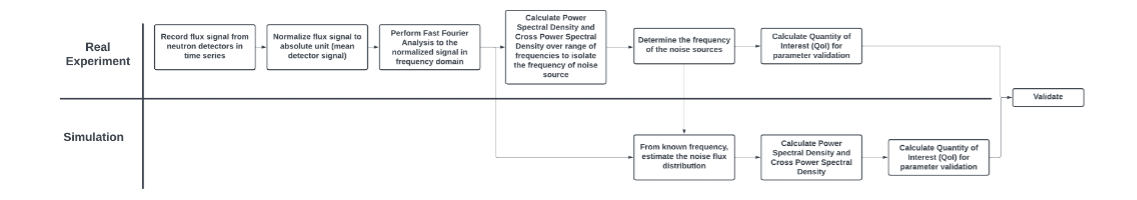
\includegraphics[width=\textwidth]{figures/ch1_Picture1.png}
        \caption{General workflow of neutron noise experiment and simulation}
        \label{fig:flow_diagram}
\end{figure}

Assuming $\delta \phi_g (\textbf{r},\omega)$ is known from the computational method, the PSD can be determined using Welch method as follow \cite{mylonakisCORESIMSIMULATIONS2021}:

\begin{equation}
        \text{CPSD}_{xy} = \biggl(\frac{\delta \phi_{g}(\textbf{r}, \omega)}{\phi_{g}(\textbf{r})} \biggr)_x^* \cdot \biggl(\frac{\delta \phi_{g}(\textbf{r}, \omega)}{\phi_{g}(\textbf{r})} \biggr)_y
        \label{eq:CPSD_comp}
\end{equation}

To further understand the physical meaning of neutron noise, we can utilize point kinetic approximations to extract the integral parameters that characterize the reactor. To do this, we start by factorizing the time-dependent forward flux into its amplitude and shape function. Such that,
\begin{equation}
        \phi (\textbf{r}, E, t) = P(t) \psi (\textbf{r}, E, t)
\end{equation}
with the following normalization condition,
\begin{equation}\label{eq:normalization}
        \frac{\partial}{\partial t} \int_{\textbf{E}} \int_{\textbf{r}} \biggl( \frac{1}{v} \phi^{\dagger}(\textbf{r}, E) \psi (\textbf{r}, E, t) \biggr) d\textbf{r} dE = 0
\end{equation}
In this case, $\phi^{\dagger}(\textbf{r})$ is the solution of the adjoint equation. 

Then, we split all the time-dependent components into the main values and the perturbations. Here, we define the initial condition (mean value) of the forward flux as follows,
\begin{equation}
        \phi_0(\textbf{r}, E) = P_0 \psi_0 (\textbf{r}, E)
\end{equation}
Therefore, we can write the noise flux as follows (neglecting second-order terms),
\begin{equation}
        \begin{aligned}
                \delta \phi(\textbf{r}, E, t) &= \phi (\textbf{r}, E, t) - \phi_0(\textbf{r}, E)\\
                &= \biggl( P_0 + \delta P(t) \biggr) \biggl( \frac{\phi_0(\textbf{r}, E)}{P_0} + \delta P(t) \biggr) - \phi_0(\textbf{r}, E) \\
                &= \phi_0(\textbf{r}, E) \frac{ \delta P(t)}{P_0} + P_0 \delta \psi(\textbf{r}, E, t)
        \end{aligned}
        \label{eq:noise_component_time}
\end{equation}
Applying Fourier transforms to Equation \ref{eq:noise_component_time} yields the following.
\begin{equation}\label{eq:noise_component_freq}
        \delta \phi(\textbf{r}, E, \omega) = \phi_0(\textbf{r}, E) \frac{ \delta P(\omega)}{P_0} + P_0 \delta \psi(\textbf{r}, E, \omega)
\end{equation}

Equation \ref{eq:noise_component_freq} shows that the noise flux can be split into two components. The first term on the right-hand side is the point-kinetic term, and the second is the spatial component of the noise flux.

The value of power perturbation can be determined as follows. We can multiply Eq \ref{eq:noise_component_freq} by $\phi^{\dagger}(\textbf{r})/v$ and integrate over all the spatial and energy domains, which leads to the following.
\begin{equation}
        \int_{\textbf{E}} \int_{\textbf{r}} \frac{1}{v} \phi^{\dagger}(\textbf{r}, E) \delta \phi(\textbf{r}, E, \omega) d\textbf{r} dE = \frac{ \delta P(\omega)}{P_0} \int_{\textbf{E}} \int_{\textbf{r}} \frac{1}{v} \phi^{\dagger}(\textbf{r}, E) \phi_0(\textbf{r}, E) d\textbf{r} dE + P_0 \int_{\textbf{E}} \int_{\textbf{r}} \frac{1}{v} \phi^{\dagger}(\textbf{r}, E) \delta \psi(\textbf{r}, E, \omega) d\textbf{r} dE
\end{equation}

Notice that due to the normalization in Equation \ref{eq:normalization} and the initial condition of the system, $\delta \psi(\textbf{r}, 0) = 0$ \cite{demaziereDevelopmentPointkineticVerification2017}. This yields to the following.
\begin{equation}
        \frac{ \delta P(\omega)}{P_0} = \frac{\int_{\textbf{E}} \int_{\textbf{r}} \frac{1}{v} \phi^{\dagger}(\textbf{r}) \delta \phi(\textbf{r}, \omega) d\textbf{r} dE}{\int_{\textbf{E}} \int_{\textbf{r}} \frac{1}{v} \phi^{\dagger}(\textbf{r}) \phi_0(\textbf{r}) d\textbf{r} dE}
\end{equation}

Continuing with the derivation of the point kinetics component, we start from time-dependent neutron diffusion equation, multiply both sides with adjoint fluxes as a weighting function, and integrate over the spatial domain, yielding the following.
\begin{equation}
    \begin{aligned}
        \frac{dP_0}{dt} + \frac{d(\delta P(t))}{dt} &= \frac{\rho_0}{\Lambda} (P_0 + \delta P(t)) + \frac{\delta \rho(t)}{\Lambda} (P_0 + \delta P(t)) - \frac{\beta}{\Lambda} (P_0 + \delta P(t)) + \lambda (C_0 + \delta C(t))\\
        \frac{dC_0}{dt} + \frac{d(\delta C(t))}{dt} &= \frac{\beta}{\Lambda} (P_0 + \delta P(t)) - \lambda (C_0 + \delta C(t))\\
    \end{aligned}
\end{equation}

By neglecting second-order terms and eliminating the time-independent component, we can simplify the equation into:
\begin{equation}
    \begin{aligned}\label{eq:simple_PRKE}
        \frac{d(\delta P(t))}{dt} &= \frac{\delta \rho(t)}{\Lambda} P_0 - \frac{\beta}{\Lambda} \delta P(t) + \lambda \delta C(t)\\
        \frac{d(\delta C(t))}{dt} &= \frac{\beta}{\Lambda} \delta P(t) - \lambda \delta C(t)\\
    \end{aligned}
\end{equation}
Applying the Fourier Transform to Equation \ref{eq:simple_PRKE} yields to:
\begin{equation}
    \begin{aligned}\label{eq:simple_PRKE_omega}
        i \omega \delta P(\omega) &= \frac{P_0}{\Lambda} \delta \rho(\omega) - \frac{\beta}{\Lambda} \delta P(\omega) + \lambda \delta C(\omega)\\
        i \omega \delta C(\omega) &= \frac{\beta}{\Lambda} \delta P(\omega) - \lambda \delta C(\omega)\\
    \end{aligned}
\end{equation}
where $\omega = 2 \pi f$. Simplifying the precursor equation of Equation \ref{eq:simple_PRKE_omega}, yields:
\begin{equation}
    \begin{aligned}\label{eq:simple_PRKE_precursor}
        \delta C(\omega) &= \frac{\beta}{\Lambda (i \omega + \lambda)} \delta P(\omega)\\
    \end{aligned}
\end{equation}
Then, substituting Equation \ref{eq:simple_PRKE_precursor} to the power equation of Equation \ref{eq:simple_PRKE_omega}, yields to:
\begin{equation}
    \begin{aligned}\label{eq:simple_power_omega}
        i \omega \delta P(\omega) &= \frac{P_0}{\Lambda} \delta \rho(\omega) - \frac{\beta}{\Lambda} \delta P(\omega) + \frac{\lambda \beta}{\Lambda (i \omega + \lambda)} \delta P(\omega)\\
        \frac{P_0}{\Lambda} \delta \rho(\omega) &= \biggl( i \omega +  \frac{\beta}{\Lambda} - \frac{\lambda \beta}{\Lambda (i \omega + \lambda)} \biggr) \delta P(\omega) \\
        \delta P(\omega) &= \delta \rho(\omega)P_0 \frac{1}{\Lambda \biggl( i \omega +  \frac{\beta}{\Lambda} - \frac{\lambda \beta}{\Lambda (i \omega + \lambda)} \biggr)} \\
        \delta P(\omega) &= \delta \rho(\omega)P_0 G(\omega)\\
    \end{aligned}
\end{equation}
Since we derive Equation \ref{eq:simple_power_omega} from Equation \ref{eq:time_2}, we can explicitly define $\delta \rho(\omega)$ as follows,
\begin{equation}
        \delta \rho(\omega) = \frac{\int_{\textbf{E}} \int_{\textbf{r}} \phi^{\dagger}(\textbf{r}, E) d\textbf{S}(\textbf{r}, E, \omega) d\textbf{r} dE}{\int_{\textbf{E}} \int_{\textbf{r}} \phi^{\dagger}(\textbf{r}, E) \textbf{F}(\textbf{r}, E) d\textbf{r} dE}
\end{equation}
where $d\textbf{S}(\textbf{r}, \omega)$ is the noise source in the system, and $\textbf{F}(\textbf{r})$  is the fission source in the forward equation. This means that we have two ways to calculate the zero-power reactor transfer function $G(\omega)$. They are,
\begin{equation}
        G(\omega) = \frac{1}{\Lambda \biggl( i \omega +  \frac{\beta}{\Lambda} - \frac{\lambda \beta}{\Lambda (i \omega + \lambda)} \biggr)} = \frac{\delta P (\omega) /P_0}{\delta \rho(\omega)}
\end{equation}

The zero-power reactor transfer function is one method for observing a system's behavior during a small sinusoidal perturbation. It could also be used to check whether the reactivity feedback is as expected from the design \cite{bellNuclearReactorTheory1970}.

\subsection{Neutron Noise Models and Sources}

Neutron noise sources can generally be divided into two categories. The first category is the localized absorbers of variable strength. Although terminology specifies absorbers, these types of noise typically refer to all types of cross-sections. This includes absorption, fission, and scattering \cite{pazsitNoiseTechniquesNuclear2010}. The absorbers of variable strength can be represented as fluctuations in the macroscopic cross-section at a given fixed location $\textbf{r}_0$ and the noise sources can be expressed as:
\begin{equation}
        \delta \Sigma_x (\textbf{r}, \omega) = \gamma (\omega) \delta (\textbf{r} - \textbf{r}_0)
\end{equation}
where $\gamma (\omega)$ is the noise source strength. Generally, the strength of the noise sources might depend on the noise frequency \cite{pazsitNoiseTechniquesNuclear2010}. Some examples of this type of noise include the perturbations traveling with the coolant flow \cite{jonssonTwogroupTheoryNeutron2011} and vibration in the control rod \cite{pazsitNeutronNoiseDiagnostics1983}. In terms of modeling the noise source in a solver, the localized absorbers of variable strength can be intuitively modeled as a perturbation of cross-sections in the center of computational nodes \cite{mylonakisCORESIMFlexible2021}.

The second category is the localized vibrating absorber. The vibrating absorbers could include vibration of the fuel assembly \cite{chionisSIMULATE3KAnalysesNeutron2017} or vibration of the core barrel \cite{pazsitDevelopmentsCoreBarrelMotion2016}. In the vibration absorber, the perturbation is modeled as the displacement of the vibrating assembly from its nominal position. In a 2D case, the perturbation is defined as follows:
\begin{equation}
        \begin{aligned}
                \delta \Sigma_{a} (x, y, \omega) = &\varepsilon_x (\omega) \delta(x-a_0) (\Sigma_{a,i,j} - \Sigma_{a,i-1,j}) + \\
                &\varepsilon_x (\omega) \delta(x+a_0) (\Sigma_{a,i,j} - \Sigma_{a,i+1,j}) + \\           
                &\varepsilon_y (\omega) \delta(x-b_0) (\Sigma_{a,i,j} - \Sigma_{a,i,j+1}) + \\
                &\varepsilon_y (\omega) \delta(x+b_0) (\Sigma_{a,i,j} - \Sigma_{a,i,j-1})
        \end{aligned}
\end{equation}
where $\varepsilon_x (\omega)$ is the displacement x-axis,  $\varepsilon_y (\omega)$ is the displacement y-axis, $a_0$ and $b_0$ are the equilibrium positions at the boundary of the vibrating assembly.

If the amplitude of $\varepsilon_x (\omega)$ and $\varepsilon_y (\omega)$ significantly lower than the size of the reactor core d, then one can use a weak absorber approach. The vibrating motion of the absorber can be described as a two-dimensional problem, where the vibrating motion will move on a two-dimensional stochastic trajectory \cite{pazsitInvestigationSpaceDependentNoise1977}. The perturbation of vibrating absorbers can be represented as:
\begin{equation}
        \delta \Sigma_{a} (x, y, \omega) = \gamma \biggl( \delta (\textbf{r} - \textbf{r}_p - \varepsilon(t)) - \delta (\textbf{r} - \textbf{r}_p) \biggr)
\end{equation}
where $\textbf{r}_p$ is the equilibrium position of the rods in motion, and $\varepsilon(t)$ is the two-dimensional displacement of the rods in motion from the equilibrium position \cite{pazsitNoiseTechniquesNuclear2010}. This model is also called the $\varepsilon/d$ model. In terms of modeling the noise source in a solver, the localized vibrating absorbers can be modeled as a perturbation of cross-sections at the boundary of the vibrating region \cite{mylonakisCORESIMFlexible2021}.

\subsection{Neutron Noise Source Unfolding}

Neutron noise source unfolding is a method that is used to identify the type of noise source and locate the position at which the perturbations occur. Generally, the noise source unfolding method primarily depends on Green’s function. Hence, determining Green’s function from the neutron noise equation is necessary \cite{demaziereIdentificationLocalizationAbsorbers2005}. The following method uses Green’s function for the neutron noise unfolding.

\subsubsection{Inversion Method}

As the name suggests, the inversion method inverts Green’s function to estimate the noise sources in the system. Recalling the definition of flux perturbations:
\begin{equation}
    \delta \phi (\textbf{r},\omega) = \int_{V_p} G(\textbf{r}, \textbf{r}_p, \omega) S(\textbf{r}_p, \omega) dV_p
    \label{eq:inversion_definition}
\end{equation}
In matrix form, Equation \ref{eq:inversion_definition} can be written as matrix-vector multiplication:
\begin{equation}
    \delta \phi (\textbf{r},\omega) = G(\textbf{r}_p \rightarrow \textbf{r}, \omega) S(\textbf{r}_p, \omega)
    \label{eq:inversion_definition_matrix}
\end{equation}
Therefore, the noise source can be determined by inverting the Green’s function such that:
\begin{equation}
    S(\textbf{r}_p, \omega) = G^{-1}(\textbf{r}_p \rightarrow \textbf{r}, \omega) \delta \phi (\textbf{r},\omega) 
    \label{eq:source_inversion_matrix}
\end{equation}

Equation \ref{eq:inversion_definition_matrix} is trivial to solve if Green’s function and the flux perturbations at each computational node are known. However, in practice, only a few detectors can be used to measure the neutron flux. Thus, only a few elements of Green’s function and the flux perturbation can be obtained from the detectors. 

An alternative proposed by \cite{demaziereIdentificationLocalizationAbsorbers2005} is to interpolate the detector readings to match the vector size $\delta \phi (\textbf{r},\omega)$. In the paper, \cite{demaziereIdentificationLocalizationAbsorbers2005} assumes that the detector is sensitive to thermal neutron and the noise source is known to be a perturbation of thermal absorption cross-section. Therefore, the interpolation is written as:
\begin{equation}
    S(\textbf{r}_p, \omega) = G^{-1}(\textbf{r}_p \rightarrow \textbf{r}_{\text{interp}}, \omega) \delta \phi (\textbf{r}_{\text{interp}},\omega) 
    \label{eq:source_inversion_matrix2}
\end{equation}
where $G^{-1}(\textbf{r}_p \rightarrow \textbf{r}_{\text{interp}}$ has size $N \times N$, $\delta \phi (\textbf{r}_{\text{interp}},\omega)$ has size $N$, and $S(\textbf{r}_p, \omega)$ has size $N$.

Using an interpolation method, \cite{demaziereIdentificationLocalizationAbsorbers2005} were able to reconstruct the noise source using an interpolation method. However, the inversion might have some problems in the boundaries because the interpolated thermal flux perturbation is forced to be equal to zero outside the reflector nodes. Even though the reconstruction at the boundaries produced poor approximation, the overall process is still providing promising results. The result of this method is highly dependent on the interpolation process. Incorrect interpolation would lead to inaccuracies in the unfolding.

\subsubsection{Zoning Method}

The zoning method is an extension of the inversion method. The difference between the two lies in using zones in the zoning method instead of interpolation. If one assumes that the system is divided into several zones $Z_k$, where each of the zones has the same number of detectors, then the flux perturbation can be written as \cite{demaziereIdentificationLocalizationAbsorbers2005}:

\begin{equation}
    \delta \phi (\textbf{r}_{\text{meas}},\omega) = \sum_{k} G(\textbf{r}_{Z_k} \rightarrow \textbf{r}_{\text{meas}}, \omega) S(\textbf{r}_{Z_k}, \omega)
    \label{eq:zoning_definition}
\end{equation}
Note that all of the $G(\textbf{r}_{Z_k} \rightarrow \textbf{r}_{\text{meas}}, \omega)$ are square matrices since $\delta \phi (\textbf{r}_{\text{meas}},\omega)$ and $S(\textbf{r}_{Z_k}, \omega)$ have the same size (number of detectors).

If the fuel assemblies represented in the zone $Z_k$ are set not to be close to each other, the response of the thermal flux detector will be unique to each other. Having the fuel assemblies belonging to a given zone $Z_k$ evenly distributed throughout the core is an easy and practical way to achieve such a goal.

Then, by inverting one of the matrices $G(\textbf{r}_{Z_k} \rightarrow \textbf{r}_{\text{meas}}, \omega)$ for zone $Z_l$, one can obtain:
\begin{equation}
    G^{-1}(\textbf{r}_{Z_l} \rightarrow \textbf{r}_{\text{meas}}, \omega) \times \delta \phi (\textbf{r}_{\text{meas}},\omega) = G^{-1}(\textbf{r}_{Z_l} \rightarrow \textbf{r}_{\text{meas}}, \omega) \biggl(\sum_{k} G(\textbf{r}_{Z_k} \rightarrow \textbf{r}_{\text{meas}}, \omega) S(\textbf{r}_{Z_k}, \omega) \biggr) + S(\textbf{r}_{Z_l}, \omega)
    \label{eq:zoning_definition_2}
\end{equation}
Moving forward, we will assume that the noise source is located at $Z_s$, which might be at one of the $Z_k$ or at $Z_l$. We have two possible cases:
\begin{enumerate}
    \item If the noise source is located at the zone $ Z_l=Z_s$, then one can write:
    \begin{equation}
        G^{-1}(\textbf{r}_{Z_l} \rightarrow \textbf{r}_{\text{meas}}, \omega) \times \delta \phi (\textbf{r}_{\text{meas}},\omega) = S(\textbf{r}_{Z_l}, \omega)
        \label{eq:zoning_case1}
    \end{equation}
    In this case, $S(\textbf{r}_{Z_l}) = S(\textbf{r}_{Z_s})$ is the “true” noise source vector. The noise source vector would have a distinct peak from any other zone, indicating that the noise source is in the zone $Z_l$. 

    \item If the inversion is done to the matrix corresponding to zone $Z_l \neq Z_s$ (contains no noise source), then Equation \ref{eq:zoning_definition_2} becomes:
    \begin{equation}
        G^{-1}(\textbf{r}_{Z_l} \rightarrow \textbf{r}_{\text{meas}}, \omega) \times \delta \phi (\textbf{r}_{\text{meas}},\omega) = G^{-1}(\textbf{r}_{Z_l} \rightarrow \textbf{r}_{\text{meas}}, \omega) G(\textbf{r}_{Z_k} \rightarrow \textbf{r}_{\text{meas}}, \omega) S(\textbf{r}_{Z_k}, \omega)        
        \label{eq:zoning_case2}
    \end{equation}
    This means that the zone $Z_l$ does not contain the noise source vector. The right-hand side of the equation will be relatively flat and no peak will be visible \cite{demaziereIdentificationLocalizationAbsorbers2005}.
\end{enumerate}

To simplify the analysis, we can perform the following calculation.
\begin{equation}
    G^{-1}(\textbf{r}_{Z_l} \rightarrow \textbf{r}_{\text{meas}}, \omega) \times \delta \phi (\textbf{r}_{\text{meas}},\omega) = S_{\text{fict}}(\textbf{r}_{Z_l}, \omega)
    \label{eq:zoning_simple}
\end{equation}
where $Z_l \in Z_k$. This calculation is done for every zone, which results in $k$ number of $S_{\text{fict}}(\textbf{r}_{Z_l}, \omega)$. For each $S_{\text{fict}}(\textbf{r}_{Z_l}, \omega)$, it should return to one of the either cases. If the zone $Z_l$ If the signal contains a noise source, then one of the vector elements should be significantly higher than the others. On the other hand, if a zone $Z_l$ does not contain a noise source, the elements of $S_{\text{fict}}(\textbf{r}_{Z_l}, \omega)$ would not be different from each other.

The zoning method generally improves the accuracy of the noise unfolding. Some errors were detected when the noise source was located near the boundary of several detectors. In this location, the detector response will not be unique to each other, making the Green’s function inaccurate \cite{demaziereIdentificationLocalizationAbsorbers2005}.

\subsubsection{Scanning method}

The third method is the scanning method. This method compares the perturbations detected by the detector with the calculated response for all possible locations of the noise source within the system. The noise source is accurately identified when the calculated neutron noise matches the measured neutron noise \cite{demaziereIdentificationLocalizationAbsorbers2005}. This method was developed by \cite{karlssonLocalizationChannelInstability1999}, and extended by \cite{demaziereDevelopmentNoisebasedMethod2002}. Both investigations successfully determined the location of the unseated fuel assembly in the Swedish Forsmark-1 BWR. Both use Green’s function as the means to compare detector readings.

This method starts with the definition of noise flux at a given location r induced by a noise source located at the location $\textbf{r}_p$ as follows:
\begin{equation}
    \delta \phi (\textbf{r}_i,\omega) = G(\textbf{r}_{p,j} \rightarrow \textbf{r}_i, \omega) S(\textbf{r}_{p,j}, \omega)
    \label{eq:scanning_definition_matrix}
\end{equation}
Using Equation \ref{eq:scanning_definition_matrix} to compare with the detector reading will be difficult since the location and strength of the noise are unknown. If one has access to two detectors at locations A and B, the ratio between the neutron noise at these two locations can be used to eliminate the noise source strength:
\begin{equation}
    \frac{\delta \phi (\textbf{r}_A,\omega)}{\delta \phi (\textbf{r}_B,\omega)} = \frac{G(\textbf{r}_{p,j} \rightarrow \textbf{r}_A, \omega)}{G(\textbf{r}_{p,j} \rightarrow \textbf{r}_B, \omega)}
    \label{eq:scanning_definition_frac}
\end{equation}

Then, the scanning algorithm consists of minimizing the following,
\begin{equation}
    \Delta(\textbf{r}) = \mathlarger{\mathlarger{\sum}}_{A,B} \biggl| \frac{\delta \phi (\textbf{r}_A,\omega)}{\delta \phi (\textbf{r}_B,\omega)} - \frac{G(\textbf{r}_{p,j} \rightarrow \textbf{r}_A, \omega)}{G(\textbf{r}_{p,j} \rightarrow \textbf{r}_B, \omega)} \biggr|
    \label{eq:scanning_definition_min}
\end{equation}
Equation \ref{eq:scanning_definition_min} implies that the summation is done for all detector pairs for all locations $\textbf{r}$. If there exist $n$ number of detectors in the reactor, thus the number of detector pairs are as follows:
\begin{equation}
    N_{\text{detector pair}} = \frac{n \times (n+1)}{2}
\end{equation}
The location at which the minimum value of $\Delta(\textbf{r})$ is found indicates the location of the noise source. The magnitude of the noise source can be calculated as follows:
\begin{equation}
    S(\textbf{r}_p,\omega) = \frac{\delta \phi(r_m,\omega)}{G(\textbf{r}_{p} \rightarrow r_m, \omega)}
\end{equation}
for any detector m.

The results from \cite{demaziereDevelopmentNoisebasedMethod2002} show that the scanning algorithm was able to locate any noise source correctly, provided there is no background. The drawback of this method is that it requires more computational power to compare every possible location of the noise source with every combination of detectors used for the evaluation.

\section{Application to Reactor Diagnostics}

The theory of neutron noise has been applied in various nuclear reactors by utilizing the noise characteristics of these reactors. The reference \cite{thiePowerReactorNoise1981} explained several reasons for using noise analysis in nuclear reactors. This includes the capability to perform specific measurements, design, or model verification, as well as simplicity, low cost, and no interference with operating procedures. Noise can also be used as a substitute for another test or inspection. The use of neutron noise analysis varies depending on the specific interest it is intended for \cite{torresNeutronNoiseAnalysis2019}. However, neutron noise theory is widely used for sensor surveillance \cite{hashemianMeasurementDynamicTemperatures2011, hashemianPracticalReviewMethods2010, montalvoAdvancedSurveillanceResistance2014}, core monitoring \cite{czibokRegularNeutronNoise2003, hashemianOnlineMonitoringApplications2011, ortiz-villafuerteBWROnlineMonitoring2006}, and core diagnostics \cite{pazsitDevelopmentsCoreBarrelMotion2016, montalvoFirstEvidencePivotal2016}. Table \ref{table:diagnostics} provides examples of noise analysis applications for various reactor types.

\begin{table}[h]
        \centering
        \caption{Some examples of noise application for power reactors}
        \begin{tabular}{ | m{3.5cm} |c| m{7cm} |c| } 
         \hline
         \textbf{Reactor Name} & \textbf{Type} & \textbf{Application}& \textbf{References} \\ 
         \hline
         Novovoronezh-1 & PWR &  Excessive looseness in the thermal shield & \cite{thiePowerReactorNoise1981} \\ 
         \hline
         Fukushima Daiichi-2 & BWR & Flow impingement caused excessive tube vibration & \cite{behringerObservationIncoreInstrument1977, mathisCharacterizationStudiesBWR41977}\\ 
         \hline
         Dresden & BWR & Monitor stability during startup & \cite{thieElementaryMethodsReactor1963} \\ 
         \hline
         Palisades & PWR & Detection of excessive and damaging flow-induced core barrel motion & \cite{fryAnalysisNeutrondensityOscillations1975} \\ 
         \hline
         High Flux Isotope Reactor (HFIR) & Research & Problems with abnormally loose control rods & \cite{behringerObservationIncoreInstrument1977, mathisCharacterizationStudiesBWR41977}\\ 
         \hline
         Experimental Breeder Reactor-1 (EBR-1) & FBR & Oscillatory fuel motion & \cite{thiePowerReactorNoise1981} \\ 
         \hline
         Dounreay Fast Reactor & FBR & Problems with abnormally loose control rods & \cite{barclayDevelopmentNoiseAnalysis1977} \\ 
         \hline
         Fort St. Vrain & Gas-cooled & Problems with motion of the core structure & \cite{thiePowerReactorNoise1981} \\ 
         \hline
         Browns Ferry-2 & BWR & Flow impingement caused excessive tube vibration & \cite{behringerObservationIncoreInstrument1977, mathisCharacterizationStudiesBWR41977} \\ 
         \hline
         Vermont Yankee & BWR & Flow impingement caused excessive tube vibration & \cite{behringerObservationIncoreInstrument1977, mathisCharacterizationStudiesBWR41977} \\ 
         \hline
        \end{tabular}
        \label{table:diagnostics}
\end{table}

In the context of core monitoring and surveillance, one example is core barrel motion (CBM) monitoring \cite{pazsitDevelopmentsCoreBarrelMotion2016}. This paper develops a methodology for investigating, diagnosing, and surveilling CBM. The surveillance was conducted at the core of Ringhals 2-4 in Sweden by inspecting the amplitude of the peaks in the normalized auto power spectral densities (APSDs) of the ex-core neutron detectors.

In this instance, the CBM was employed because visible vibrations were detected in the radial supports of the core barrel in the Ringhals reactors. In \cite{martinSURVEILLANCEDIAGNOSTICSBEAM2012}, the investigation focuses on the pendulum motion of the core barrel, or it is also known as the beam mode. During the Ringhals operation, monitoring of the beam mode indicated that the amplitude of the APSD increased throughout the fuel cycle. However, the APSD decreased after the refueling \cite{pazsitFinalReportResearch2011}. 

In the context of reactor core diagnostics, noise analysis is useful for analyzing situations that require changes in state variables, as these changes affect the reactor's status. This was demonstrated in \cite{demaziereDevelopmentNonintrusiveMethod2002} by measuring the moderator temperature coefficient (MTC). Traditionally, at-power MTC measurement techniques require the reactor to be perturbed to induce the change of the moderator temperature. The implementation of the direct perturbation method is the MTC measurement at the Righals-4 reactor using the boron dilution method. The result of this method shows that the uncertainty of using boron dilution method was much more significant than expected due to the necessary reactivity corrections. This prompted the use of non-intrusive methods such as noise analysis for reactor diagnostics.

Some noise experiments were done in two research reactors (AKR-2 and CROCUS) using two different types of neutron noise. The first type of perturbation was generated by a rotating neutron absorber with a varying absorption cross-section with respect to the rotation angle and the second one by fuel rods that oscillate in a controlled manner inside the reactor core \cite{lamirandExperimentalReport1st2018, lamirandExperimentalReport2nd2021, lamirandExperimentalReport3rd2021}. The experiments consisted of two different parts representing different sources of periodic reactivity perturbation that created neutron flux oscillations. The experiments produced two different quantities of interest: the spectral power density (SPD) and the phase shift angle between detector pairs \cite{ambrozicNoiseAnalysisTechniques2020}. 

AKR-2 reactor is a thermal, homogeneous, polyethylene-moderated zero-power reactor located at TU Dresden. For the first type of experiment in AKR-2, a piece of Cadmium is rotated in the reactor core. Cadmium was chosen due to the variable absorption reaction rate with respect to the rotation angle \cite{hubnerEXPERIMENTALDETERMINATIONZERO2021}. For the second type of experiment in AKR-2, the mechanical vibration consists of a neutron absorber that moves linearly back and forth in an experimental channel located outside of the reactor core \cite{lamirandExperimentalReport1st2018}. The CROCUS reactor is an experimental reactor dedicated to research and teaching in radiation and reactor physics, located at the École Polytechnique Fédérale de Lausanne (EPFL). For noise analysis, the CROCUS reactor used the COLIBRI experimental setup consisting of a fuel rod oscillator and neutron detection instrumentation \cite{lamirandExperimentalReport1st2018, lamirandExperimentalReport2nd2021, lamirandExperimentalReport3rd2021, lamirandCOLIBRIExperimentalProgram2020}. 

In terms of modeling validation, the CORTEX (COre monitoring Techniques: EXperimental validation and Demonstration) project used two approaches to implement noise analysis based on a given noise source \cite{demaziereCORTEXProjectImproving2020}. The first approach uses the formulation of the linearized neutron noise equation in the frequency domain. From the equation, the neutron noise can be determined as a complex quantity. The second approach calculates the evolution of the spatial distribution of the flux as a function of time by solving the time-dependent neutron transport equation \cite{hursinModelingNoiseExperiments2023, brighentiDevelopmentValidationTimedependent2022}. 

The CORTEX project concluded in 2021; its final phase involves implementing commercial nuclear power plants (NPPs). This is done by demonstrating the approaches to four different commercial reactors. Four reactors are used for the demonstration exercises: a German four-loop pre-Konvoi PWR, a Swiss three-loop pre-Konvoi PWR, a Czech VVER-1000 reactor, and a Hungarian VVER-440 reactor \cite{demaziereCORTEXProjectImproving2020, seidlReviewHistoricNeutron2015}. For the German pre-Konvoi and Konvoi-type PWR, noise measurement and analysis have been topics of interest for several years. Numerous noise observations have been conducted on both reactors during the commissioning and operational phases. It has been observed that during its 30-year operation, fluctuations in neutron noise signals have occurred. These were mainly low-frequency neutron noise, which could cause problems for future reactor operations. Some knowledge of neutron noise and the reactor's operation is necessary to solve the problem \cite{seidlReviewHistoricNeutron2015, rohdeNeutronNoiseObservations2018}.

\section{Computational Methods and Tools of Neutron Noise Analysis}

\subsection{Solving Neutron Noise Problems using Deterministic Methods}

Building on the success of neutron noise experiments, computational methods and tools are being developed to support neutron noise's validation and verification efforts. Deterministic transport methods have been developed to solve the neutron noise equation. It should be noted that knowledge of the forward neutron flux distribution and k-criticality is necessary to perform neutron noise simulations, as these parameters become the input to the neutron noise simulation \cite{demaziereDevelopment2D2group2004}. The tools developed varied in terms of spatial discretization, energy discretization, angular discretization, and the domain of interest to solve the neutron noise equation. 

Diffusion theory is the most widely used approximation in existing tools. Although diffusion theory employs the most approximations compared to other methods for solving the neutron transport equation, it is still deemed compatible with the analysis \cite{duderstadtNuclearReactorAnalysis1977, demaziereNumericalToolsApplied2009}. Some of the first developments of neutron noise simulators based on neutron diffusion theory are \cite{kherichaDevelopmentTwoenergyGroup2001} and \cite{demaziereDevelopment2D2group2004}. The development of the noise simulator began with the need for a dynamic calculation to determine the dynamic reactor transfer function. In the past, calculations of dynamic reactor transfer functions have been performed. However, these calculations are only for a few homogeneous regions. In \cite{kherichaDevelopmentTwoenergyGroup2001}, a 2-group, 2-dimensional Neutron noise simulator based on the nodal method is proposed. The simulator calculates the frequency-dependent detector (adjoint function). Since the simulator employs nodal methods, an iteration procedure is necessary to achieve convergence. In \cite{demaziereDevelopment2D2group2004}, the noise simulator is developed to solve neutron noise problems using both forward and adjoint approaches. In contrast to \cite{kherichaDevelopmentTwoenergyGroup2001}, the noise simulator in \cite{demaziereDevelopment2D2group2004} uses a finite difference scheme for the spatial discretization. By using a finite difference scheme, the need for an iteration procedure is eliminated. In both simulators, the noise simulator is coupled using a static simulator. Some cases are simulated to verify the capability of the noise simulators. Namely, noise simulators use the vibration and absorber strength case for verification. Subsequently, efforts have been made to enhance the accuracy of the noise simulator. One of the efforts is to use the analytical nodal method \cite{smithAnalyticNodalMethod1979} to solve the Neutron noise equation. This represents an improvement over using the finite difference scheme for spatial discretization \cite{larssonNeutronNoiseCalculations2011}. In \cite{larssonNeutronNoiseCalculations2011}, the analytical nodal method is used for both forward flux and neutron noise calculations. Other tools, such as CORE SIM \cite{demaziereCORESIMMultipurpose2011, dykinDEMONSTRATIONCOUPLEDCORE2014} and CORE SIM+ \cite{mylonakisCORESIMFlexible2021, mylonakisNeutronNoiseModelling2019, mylonakisNumericalSolutionTwoenergygroup2020}, are designed to address the neutron noise equation. These specialized codes employ the 3-dimensional, 2-group neutron diffusion equation as the foundational framework for solving the Neutron noise equation in the frequency domain. Notably, these codes exhibit the ability to simulate both critical and subcritical systems, expanding their utility and versatility. Their prowess in handling such systems empowers them to calculate the static flux within the software and then leverage this static flux information to derive dynamic solutions. Moreover, these codes have the capability to solve Green's functions numerically, further enhancing their computational efficiency and versatility.

As the system of interest becomes more complicated and heterogeneous, one could argue that the approaches mentioned in the previous paragraph are insufficient to solve these problems. Seeing this problem, deterministic codes such as APOLLO3 and SIMULATE-3K developed a noise solver in their system of codes \cite{chionisSIMULATE3KAnalysesNeutron2017, rouchonNew3DMultigroup2017}. However, some other developers argue that diffusion theory is insufficient to solve the neutron noise equation. Some disadvantages of using diffusion theory to solve the Neutron noise equation include the incapability of diffusion theory to describe the anisotropy of neutron density in the system, and the use of a time-dependent diffusion equation is deemed inadequate to solve neutron noise equation, since the parabolic nature of diffusion equation results in the particles having an infinite velocity \cite{bellNuclearReactorTheory1970, bahramiSNTransportMethod2018}. Therefore, more accurate methods are developed to solve the Neutron noise equation deterministically. One example is to use the P1 approximations to verify the assumptions and approximations used in diffusion theory-based noise simulators \cite{pazsitNeutronNoiseTheory2002, larssonComparativeStudy2group2009}. The use of P1 approximations for noise simulators stems from the fact that both static and dynamic perturbations in noise systems are non-isotropic sources in the subcritical system. Therefore, the solutions of the forward angular flux and the angular noise could be expanded using P1 expansion to consider this behavior. In \cite{pazsitNeutronNoiseTheory2002}, it is understood that the P1 approximations of a one group noise equation would lead to some difference in noise scenarios. For the case where the perturbation affects only the absorption cross-section (localized absorber and absorption of variable strength cases), the difference between using diffusion and P1 approximation is negligible. However, when perturbations affect the scattering cross-section, the difference between using the diffusion and P1 approximations is significant. The noise source would become a noise field. This is understandable, as the P1 approximation affects the assumptions underlying the definition of the scattering term in the neutron transport equation and the neutron noise equation. In \cite{larssonComparativeStudy2group2009} the difference between the P1 approximation and diffusion theory would not be negligible in a heterogeneous system, especially in the near-interface regions where the static flux between the two approximations differs.

Other deterministic methods that are used to solve the neutron noise equation are the simplified P3 method \cite{brantleySimplifiedApproximation2000, gongNeutronNoiseCalculation2021}, discrete ordinate method \cite{bahramiSNTransportMethod2018, yiSimulationNeutronNoise2021}, and random ray method \cite{cosgroveMemoryefficientNeutronNoise2024}. For the simplified P3 method, \cite{gongNeutronNoiseCalculation2021} investigate the differences in implementation and results compared to the diffusion approximations. Compared to the general PN Equation, the Simplified PN replaces the second derivatives of angular flux moments in the one-dimensional planar geometry PN equation into general three-dimensional Laplacian operators \cite{brantleySimplifiedApproximation2000}. The simplified P3 method is implemented in the industry-standard SP3 solver, CORCA-PIN, which is modified into a prototype code, CORCA-NOISE. Compared to the diffusion approximations, the simplified P3 approximations exhibit a considerable difference when applied to heterogeneous reactors, such as the MOX core. For the discrete ordinate method, a solver called NOISE-SN was developed \cite{yiSimulationNeutronNoise2021}. NOISE-SN simulates Neutron noise problems in the frequency domain. When applying the discrete ordinate method, it is essential to note that the discretization of the angular variable cannot account for all directions of neutron travel. Therefore, it will create the so-called ray effect. The ray effect refers to the anomalous oscillations of the scalar and angular fluxes that occur in certain numerical calculations \cite{lathropRayEffectsDiscrete1968}.  The discrete ordinate method captures the spatial distribution of Neutron noise significantly better compared to diffusion approximations. This is crucial for accurately predicting the location of the noise source for diagnostic purposes \cite{bahramiPreciseLocalizationNeutron2021}. 

Several tools investigate the application of time-domain calculations to neutron noise equations. One of the tools that employs a time-domain analysis approach is FEMFFUSION \cite{vidal-ferrandizNeutronicSimulationFuel2020, vidal-ferrandizTimeFrequencyDomain2020, vidal-ferrandizModellingSimulationsReactor2022, vidal-ferrandizFEMFFUSIONFiniteElement2023}. FEMFFUSSION is a 3-dimensional, 2-group neutron diffusion simulator that uses a finite element method to solve the neutron diffusion equation \cite{vidal-ferrandizMovingMeshesSolve2016, vidal-ferrandizSolutionLambdaModes2014}. FEMFFUSION solves the neutron noise equation in the time domain and utilizes the frequency domain in the latest version of the code. The calculations in the time domain and frequency domain are then compared by applying a numerical Fast Fourier Transform (FFT) algorithm to the time-dependent results. Another tool that has been utilized for neutron noise simulation in the time domain is DYN3D \cite{viebachInfluenceDynamicalFuel2018, viebachVerificationCodeDYN3D2022}. DYN3D is a system code that solves the two-group diffusion equation in the time domain using a nodal expansion method with transverse integration for spatial dependence and considering six groups of delayed neutron precursors \cite{viebachVerificationCodeDYN3D2022}. 

It should be noted that in deterministic code, the perturbed cross-sections are not calculated directly from the neutron cross-section libraries \cite{ardiansyahEvaluationPBMR400Core2021}. Instead, these cross-sections are already a function of space, time, energy, and direction based on the mesh in which the calculation is performed. Therefore, it is essential to consider that the neutron cross-sections must be defined in advance in deterministic methods. 

\subsection{Solving Neutron Noise Problems using Monte Carlo Methods}

For neutron transport calculation, the use of Monte Carlo arises since we can treat the macroscopic cross-sections of neutrons as the probability of interactions per unit distance traveled by neutrons. The Monte Carlo method has proven effective for some cases of neutron transport, especially those related to complex geometries and variations in neutron cross-sections with energy. Monte Carlo eliminates the need for subsidiary calculations such as resonance flux and cross-section group constants \cite{bellNuclearReactorTheory1970, duderstadtNuclearReactorAnalysis1977}. In Monte Carlo, sets of neutrons are generated and simulated. For each individual neutron, the path is traced as it traveled through some materials, including the types of interactions that happened to the neutrons. The generation of neutrons, actual locations, types of interactions, and the results are all determined from a range of possibilities that are set by random numbers generated in Monte Carlo \cite{lewisComputationalMethodsNeutron1984, luxMonteCarloParticle1991}. 

With the vast capability of Monte Carlo to estimate the solution of the neutron transport equation, one would determine and test the capability of Monte Carlo to estimate the solution of the Neutron noise equation. Compared to deterministic codes, Monte Carlo estimates the neutron cross-sections from the cross-section libraries to calculate the static flux. The application of Monte Carlo to estimate the Neutron noise equation still has some challenges. In the previous section, it was determined that the Neutron noise equation in the frequency domain has some similarities with a fixed-source (or subcritical) neutron transport equation. However, some terms are different and refer to different physical phenomena in the Neutron noise equation. Comparing Equation 28 to the neutron transport equation, the first difference is on the $\delta \phi (\textbf{r}, \omega)$, which is the complex-valued variable. The second difference is in the source term of the Neutron noise equation, which contains complex-valued variables and negative signs. Finally, the difference is on the time-dependent term, which includes a complex value. In the application of Monte Carlo, these three differences mean that the particle weights W will possibly have real and imaginary values that can be either positive or negative. This is different than the conventional Monte Carlo methods, which only treat real and positive particle weights \cite{yamamotoMonteCarloMethod2013}.

With these differences, a new algorithm has been developed to solve these problems. \cite{yamamotoImplementationFrequencydomainNeutron2018} propose the use of complex particle weight such that,
\begin{equation}
    W(\omega) = (W_R (\omega), W_I (\omega))
\end{equation}
where $W_R$ is the real part of particle weight, and $W_I$ is the imaginary part of particle weight. The algorithm also includes the $ \frac{i \omega}{v} \delta \phi (\textbf{r}, \omega)$ term to the random walk process and weight cancellation of positive and negative weights. The noise source is determined using the static flux of the critical calculation and the perturbation in the cross-sections. This method has been developed in the modified MCNP code and verified using 2 group model, and BWR benchmark model.

Another algorithm proposed by \cite{rouchonNewMonteCarlo2017} chose to change the collision kernel formally, by adding a new term that contains real and complex values, $\frac{(\eta - i)}{\eta} \eta \frac{\omega}{v} \delta \phi (\textbf{r}, \omega)$, where $\eta$ is a real constant with the same sign as $\omega$. With this definition, the collision operator in the neutron noise equation is different compared to the neutron transport equation. Consequently, there will be two different types of production to be considered. The first one is the regular fission production, which is like standard neutron transport Monte Carlo calculation. The second one is the $\omega$-production associated with the scalar 'copy' operator. Just like the previous algorithm, the noise source is sampled based on the critical calculation of the flux multiplied by the perturbation of the cross-section. The perturbation of cross-sections is case-by-case, which means that different types of phenomena will have different definitions of cross-section perturbation. The second algorithm has been implemented to the Monte Carlo code Tripoli-4 \cite{rouchonNewNeutronNoise2019} and verified against an analytical solution using the infinite homogeneous medium model, infinitely long homogeneous cylindrical core, and one-dimensional homogeneous core surrounded by a reflector. More verification is also done to analyze the Neutron noise in a PWR assembly using simple noise sources and vibration-induced noise sources.

Another topic of interest in Monte Carlo application is neutron noise sampling and variance reduction, which is addressed in \cite{belangerVarianceReductionNoise2022}. In the paper, a novel method to sample the neutron noise source exactly as a perturbation of isotopic composition is introduced. This paper also addresses the variance reduction using weight cancellation during the calculation. The Monte Carlo-based method is also developed to generate the modified Green’s function as proposed in \cite{demaziereMonteCarlobasedDynamic29}. Driven by the fact that the Neutron noise problem is similar to the case of subcritical assembly with external source, Monte Carlo method is used to calculate modified Green’s functions associated to the real part of the dynamic macroscopic cross-sections. Once the modified Green’s function is determined, neutron noise induced at any location by any perturbation can be determined \cite{demaziereMonteCarlobasedDynamic29}.



\chapter{Application Neutron Noise Methods in 2D and 3D HTTR}

\section{Simulation of Neutron Noise in 2D and 3D HTTR}

\section{Application of Neutron Noise Unfolding methods for HTTR}


\chapter{Novel Neutron Noise Unfolding methods and applications}


\chapter{Conclusions}

We conclude that graduate students like coffee.

%%%%%%%%%%%%%%%%%%%%%%%%%%%%%%%%%%%%%%%%%%%%%%%%%%%%%%%%%%%%%%%%%%%%%%%%%%%%%%%
% per Graduate College preference, place the \appendix and the appendices content before the
% bibliography (here) only if the appendices contain references.
\backmatter

\printbibliography[heading=bibintoc,title={References}]

% the below lines are only needed if bibliography precedes appendices
% uses https://tex.stackexchange.com/a/440212 to continue page numbering
\clearpage
\setcounter{counterforappendices}{\value{page}}
\mainmatter
\setcounter{page}{\value{counterforappendices}}

%\appendix

%\chapter{An appendix}

%\lipsum[1-5]

% \input{Appendix.tex}

\end{document}
